\section{Use case diagram}
\subsection{Points communs}
	Etant donnée la nature des deux applications, de nombreux points communs sont à souligner dans les use cases tels que les logs, gestion des notifications et gestion des paramètres.
\newline
\newline

Concernant le système de log, cela peut s'apparenter à une application "classique" contenant des utilisateurs avec des fonctionnalités telles que créer un compte, s’authentifier, se déconnecter et réinitialiser le mot de passe.
\newline
\newline

Pour la gestion des notifications, l'utilisateur aura la possibilité de voir les détails des notifications qu'il aura reçues, de les marquer comme lues et aura le choix de les accepter ou de les refuser. De plus, l'utilisateur pourra rafraichir la page pour voir apparaitre de nouvelles notifications (de même que mentionné dans l'énoncé).
\newline
\newline

En ce qui concerne la gestion des paramètres, l’utilisateur aura notamment la possibilité de modifier son mot de passe en ayant reçu un mail de confirmation au préalable.  Au sujet de la gestion des langues, ce dernier aura le droit d'en ajouter, d'en choisir une qui sera sa langue favorite et de changer la langue actuelle de l'application.
\newline
\newline

Nous pouvons observer que le serveur est un acteur qui enregistrera toutes les informations utiles et qu’il jouera le rôle de correspondant entre le client et le fournisseur par le biais du use case : "transférer les données".
Pour permettre une meilleure lisibilité et compréhension de notre diagramme, nous avons décidé d’impliquer le serveur uniquement dans certaines actions. De ce fait, celui-ci n’est pas relié aux Use cases portant par exemple le nom de « Fermer un portefeuille ».

\newpage
\subsection{Client}

Les deux points principaux à noter sont les Use cases « Voir les portefeuilles » et « Voir les contrats ». En effet, c’est à partir de ces derniers que la logique même des fonctionnalités disponibles pour le client repose.
\newline
\newline

Lorsque le client est sur la section « Voir les portefeuilles », il pourra créer un portefeuille, fermer un portefeuille, voir les données de consommation et gérer ces données.
Il convient de signaler que nous avons décidé de créer une sous-catégorie supplémentaire "Gestion de consommation" afin d'apporter une meilleure lisibilité et séparation des sections.
\newline
\newline

Quant à la section « Voir les contrats », il aura la capacité d’ajouter ou fermer des contrats. 
En vue d’ajouter des contrats, le client devra forcément voir les fournisseurs et contrats relatifs. Nous avons choisi que cette option devra également être disponible sans se rendre dans la section mentionnée précédemment.

\begin{figure}[h]
\centering
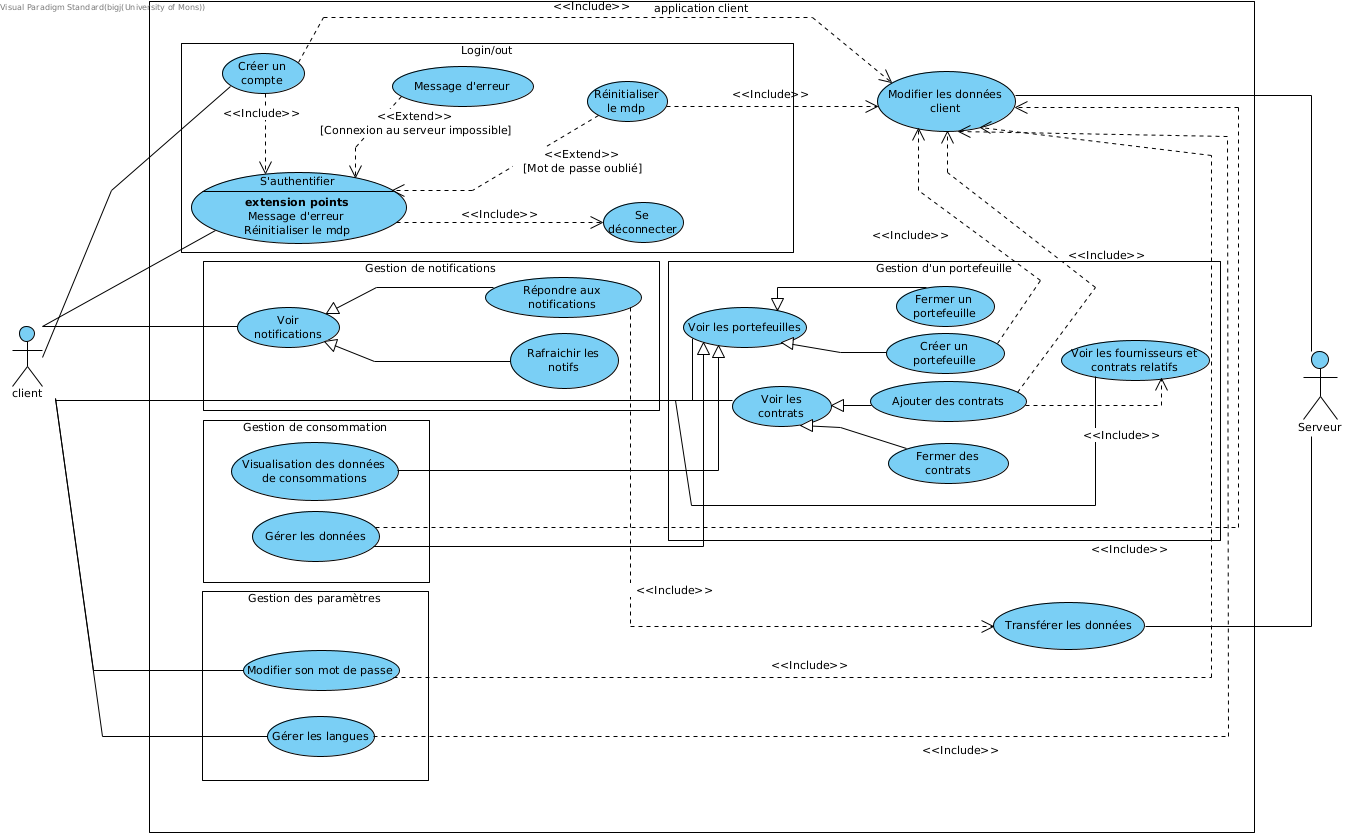
\includegraphics[width = 1\textwidth]{use_case/client.png}
\end{figure}

\newpage

\subsection{Fournisseur}

Pour le fournisseur, les principales différences résident dans le fait qu’il n’y aura plus les sections « Voir les portefeuilles » et « Voir les contrats » mais « Voir ses clients » et « Voir les contrats clients ».
\newline
\newline

Dans la même optique que pour la gestion d’un portefeuille chez le client, le fournisseur une fois sur la section « Voir ses clients » sera apte à ajouter ou supprimer un client, voir les données de ses clients ainsi que les gérer.
\newline
\newline

Ce dernier aura, de plus, la possibilité d’ajouter ou fermer des contrats et changer les paramètres des contrats sur « Voir les contrats clients ».

\begin{figure}[h]
\centering
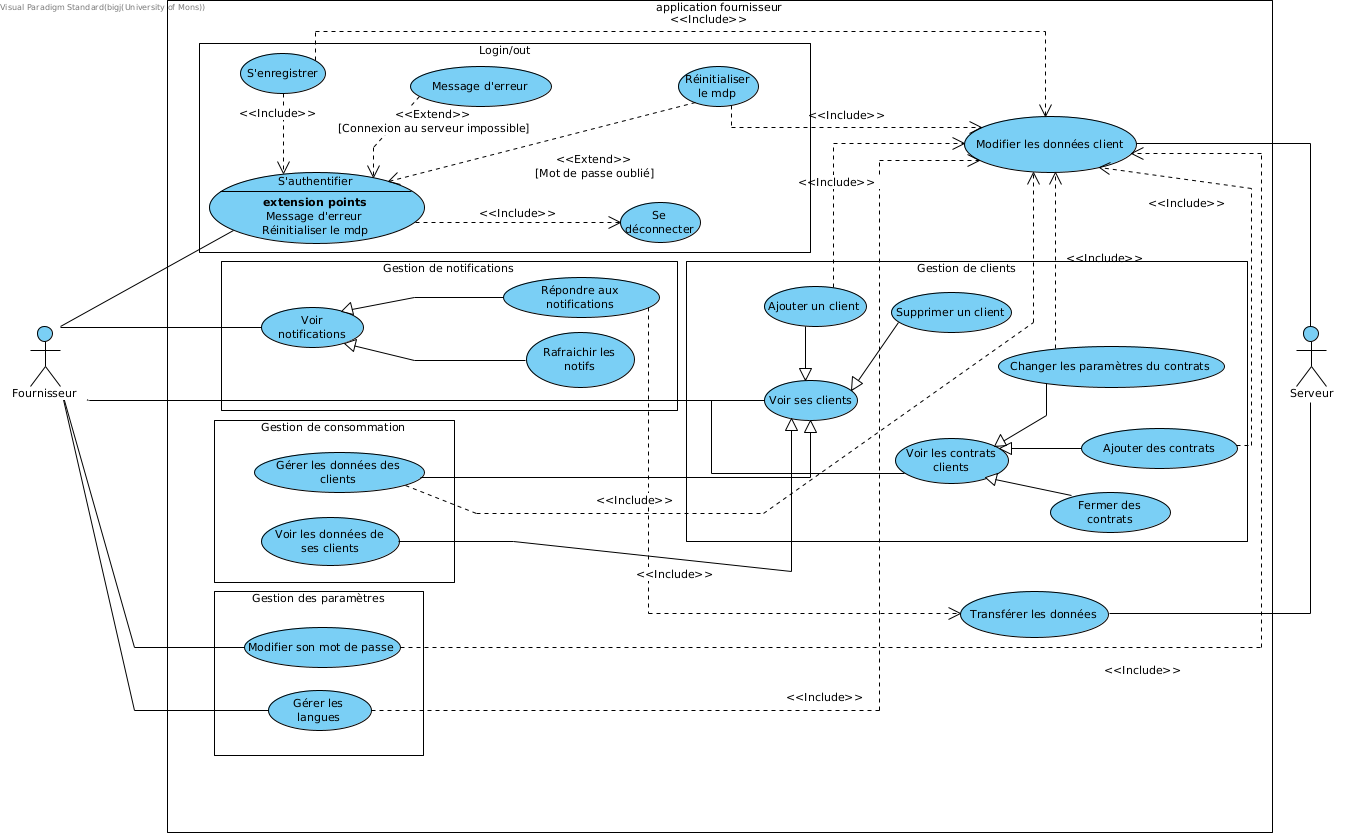
\includegraphics[width = 1\textwidth]{use_case/fournisseur.png}
\end{figure}
